\documentclass[11pt]{article}

% ---------- Packages (per course conventions) ----------
\usepackage[margin=1in]{geometry}
\usepackage{graphicx}
\usepackage{float}
\usepackage{booktabs}
\usepackage{siunitx}
\usepackage{amsmath}
\usepackage{amssymb}
\usepackage{tikz}
\usepackage{tcolorbox}
\usepackage{xcolor}
\usepackage{hyperref}
\hypersetup{colorlinks=true, linkcolor=black, urlcolor=blue}

\setlength{\parindent}{0pt}
\setlength{\parskip}{\baselineskip}

\DeclareSIUnit{\lb}{lb}
\DeclareSIUnit{\ft}{ft}
\DeclareSIUnit{\kN}{kN}

% ---------- TikZ styles and FBD helpers ----------
\usetikzlibrary{arrows.meta,calc,patterns}
\tikzset{
  member/.style={line width=2.6pt, draw=cyan!35!blue!55!black, line cap=round, line join=round},
  pin/.style={circle, draw=black, fill=white, inner sep=0pt, minimum size=5pt, line width=0.8pt},
  load/.style={-{Latex[length=2.8mm,width=2mm]}, line width=1.2pt, red!75!black},
  rxn/.style={-{Latex[length=2.8mm,width=2mm]}, line width=1.2pt, blue!75!black},
  couple/.style={-{Latex[length=2.4mm,width=1.8mm]}{Latex[length=2.4mm,width=1.8mm]}, line width=1.2pt, blue!75!black},
  mf/.style={-{Latex[length=2.6mm,width=1.9mm]}, line width=1.1pt, black!85},
  dim/.style={{Latex[length=1.7mm,width=1.2mm]}-{Latex[length=1.7mm,width=1.2mm]}, line width=0.4pt, black!60},
  ext/.style={line width=0.3pt, black!40},
  axis/.style={-{Latex[length=2mm]}, line width=0.5pt, black!55},
  dl/.style={font=\footnotesize, fill=white, inner sep=1pt},
}
% ---------- joint FBD helpers ----------
% \jfbd{caption}{body}: joint at origin, members drawn as arrows pointing away (tension assumed)
\newcommand{\jfbd}[2]{\begin{tikzpicture}[baseline=(cap.base)]
  \path[use as bounding box] (-2.15,-1.95) rectangle (2.15,1.65);
  #2
  \node[pin, minimum size=7pt] at (0,0) {};
  \node[font=\footnotesize\bfseries] (cap) at (0,-1.8) {#1};
\end{tikzpicture}}
% member force (unknown, tension assumed): \mT{angle}{label}
\newcommand{\mT}[2]{\pgfmathsetmacro{\anc}{#1+180}%
  \draw[mf] (#1:0.14) -- (#1:1.05);
  \node[font=\footnotesize, inner sep=1.5pt, anchor=\anc] at (#1:1.05) {#2};}
% known force acting away from the joint: \fout{angle}{label}
\newcommand{\fout}[2]{\pgfmathsetmacro{\anc}{#1+180}%
  \draw[load] (#1:0.14) -- (#1:1.05);
  \node[font=\footnotesize, inner sep=1.5pt, anchor=\anc] at (#1:1.05) {#2};}
% known force pushing into the joint, tail at "angle": \fin{angle}{label}
\newcommand{\fin}[2]{\pgfmathsetmacro{\anc}{#1+180}%
  \draw[load] (#1:1.05) -- (#1:0.16);
  \node[font=\footnotesize, inner sep=1.5pt, anchor=\anc] at (#1:1.05) {#2};}
% reaction versions (blue)
\newcommand{\rout}[2]{\pgfmathsetmacro{\anc}{#1+180}%
  \draw[rxn] (#1:0.14) -- (#1:1.05);
  \node[font=\footnotesize, inner sep=1.5pt, anchor=\anc] at (#1:1.05) {#2};}
\newcommand{\rin}[2]{\pgfmathsetmacro{\anc}{#1+180}%
  \draw[rxn] (#1:1.05) -- (#1:0.16);
  \node[font=\footnotesize, inner sep=1.5pt, anchor=\anc] at (#1:1.05) {#2};}
% angle arc between a1 and a2 with label: \jang{a1}{a2}{label}
\newcommand{\jang}[3]{\draw[black!55, line width=0.4pt] (#1:0.55) arc (#1:#2:0.55);
  \pgfmathsetmacro{\mid}{(#1+#2)/2}\node[font=\scriptsize, black!70] at (\mid:0.78) {#3};}

% =========================================================
% EDIT THESE FOR EACH NEW ASSIGNMENT
% =========================================================
\newcommand{\assignmentNumber}{5}
\newcommand{\assignedDate}{16 Oct 2026}
\newcommand{\dueDate}{23 Oct 2026}
\newcommand{\numProblems}{8}

% ---------- Boxed-answer helper ----------
\newtcolorbox{finalanswer}{
    colback=white, colframe=black, boxrule=1pt,
    title=Answer, fonttitle=\bfseries, coltitle=black,
    colbacktitle=white
}

% ---------- Sketch frame ----------
\newtcolorbox{sketchframe}{colback=white, colframe=black!45, boxrule=0.5pt,
    left=4pt, right=4pt, top=6pt, bottom=4pt, before upper={\centering}}

% ---------- Problem scaffold ----------
\newcommand{\problemstart}[2]{%
    \clearpage
    \setlength{\parskip}{0.5\baselineskip}
    \setlength{\abovedisplayskip}{4pt}\setlength{\belowdisplayskip}{4pt}
    \section*{Problem #1}
    \textbf{Given / Find:} #2

    \textbf{Sketch:}
}

\begin{document}

% =========================================================
% COVERSHEET
% =========================================================
\begin{titlepage}
    \centering
    \vspace*{2cm}
    {\LARGE \bfseries ENGR 225: Mechanics 1} \\[0.3cm]
    {\Large Homework Coversheet} \\[0.3cm]
    {\large Assoc.\ Prof.\ Clayton Byers} \\[2cm]

    \begin{flushleft}
        \Large
        \textbf{NAME:} \underline{\hspace{0.5cm}Sean Balbale\hspace{4.5cm}} \\[1cm]
        \textbf{DATE:} \underline{\hspace{10cm}} \\[1cm]
        \textbf{ASSIGNMENT:} \underline{\hspace{0.5cm}Homework 5\hspace{3.5cm}} \\[2cm]
    \end{flushleft}

    \large
    \textbf{Level of involvement of AI, LLMs, or related tools in the completion of this assignment:}

    \vspace{1cm}

    \begin{flushleft}
        \Large
        $\square$ \quad None \\[0.7cm]
        $\square$ \quad Minor \\[0.7cm]
        $\square$ \quad Major \\[0.7cm]
        $\square$ \quad Extensive \\[1.5cm]
    \end{flushleft}

    \normalsize
    \textit{Mark the box that applies (e.g., replace $\square$ with $\blacksquare$, or type an X beside it, before compiling/printing). Your disclosure does not affect your grade -- it keeps you accountable for the work you are doing.}

\end{titlepage}

% =========================================================
% HOMEWORK HEADER
% =========================================================
\section*{ENGR 225 -- Homework \assignmentNumber}
\textbf{Assigned:} \assignedDate \hfill \textbf{Due:} \dueDate

In the sketches, applied loads are red, support reactions are blue, and member forces are black. I drew every member force in tension, so a negative answer means that member is in compression.

% =========================================================
% PROBLEM 1
% =========================================================
\problemstart{1}{Rod $ABC$ is held by smooth journal bearings at $A$, $B$, and $C$, which only exert forces on the rod. With $F_1=\SI{300}{\lb}$, find the magnitude of $F_2$ that makes the bearing reaction $C_y$ zero.}

\begin{sketchframe}
\scalebox{0.74}{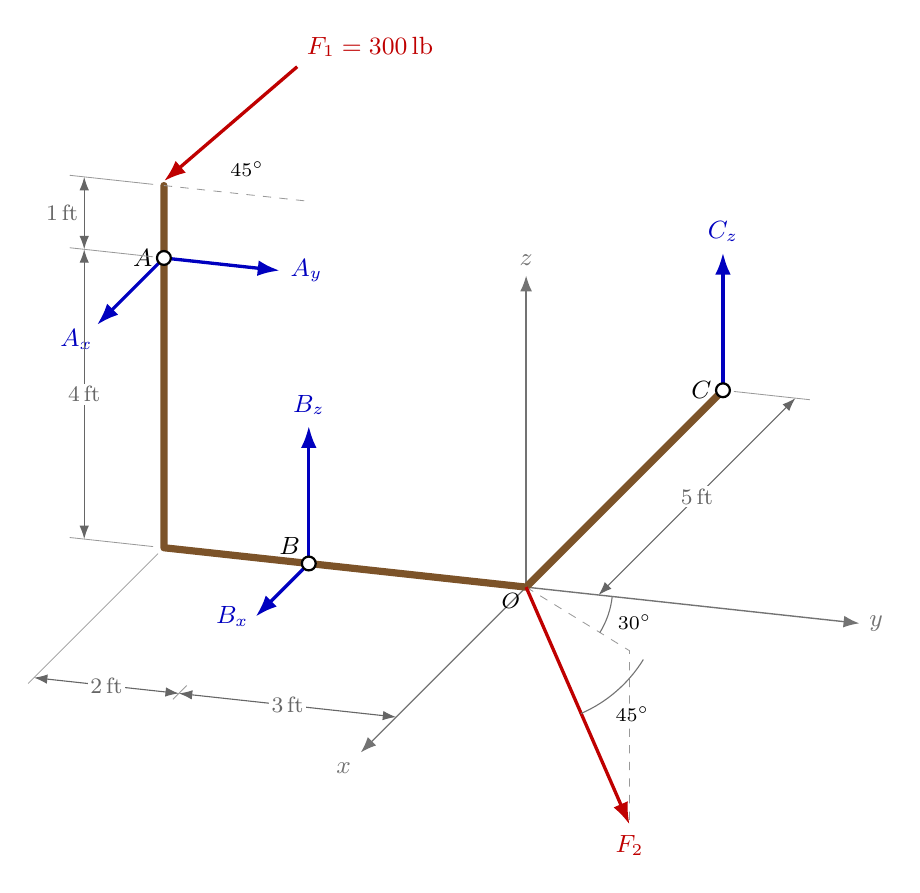
\begin{tikzpicture}[x={(-0.5cm,-0.5cm)}, y={(0.92cm,-0.1cm)}, z={(0cm,0.92cm)}, font=\small]
  % axes
  \draw[axis] (0,0,0) -- (4.2,0,0) node[below left]{$x$};
  \draw[axis] (0,0,0) -- (0,4.6,0) node[right]{$y$};
  \draw[axis] (0,0,0) -- (0,0,4.3) node[above]{$z$};
  % rod
  \draw[member, draw=brown!65!black] (-5,0,0) -- (0,0,0) -- (0,-5,0) -- (0,-5,5);
  % F1 at top of vertical leg, in the yz-plane, 45 deg below horizontal
  \draw[ext, dashed] (0,-5,5) -- (0,-3.0,5);
  \draw[load] (0,-3.16,6.84) -- (0,-5,5.06);
  \node[red!75!black, anchor=south west] at (0,-3.16,6.84) {$F_1=\SI{300}{lb}$};
  \node[font=\scriptsize] at (0,-3.85,5.35) {$45^\circ$};
  % F2 at O
  \draw[ext, dashed] (0,0,0) -- (1.2,2.08,0) -- (1.2,2.08,-2.4);
  \draw[load] (0,0,0) -- (1.2,2.08,-2.4) node[below]{$F_2$};
  \draw[black!55, line width=0.4pt] (-6.2:1.1cm) arc (-6.2:-31.7:1.1cm); \node[font=\scriptsize] at (-18:1.45cm) {$30^\circ$};
  \draw[black!55, line width=0.4pt] (-31.7:1.75cm) arc (-31.7:-66.5:1.75cm); \node[font=\scriptsize] at (-50:2.1cm) {$45^\circ$};
  % reactions (assumed positive)
  \draw[rxn] (0,-5,4) -- (1.7,-5,4) node[below left, inner sep=1pt]{$A_x$};
  \draw[rxn] (0,-5,4) -- (0,-3.4,4) node[right]{$A_y$};
  \draw[rxn] (0,-3,0) -- (1.35,-3,0) node[left, inner sep=2pt]{$B_x$};
  \draw[rxn] (0,-3,0) -- (0,-3,1.9) node[above]{$B_z$};
  \draw[rxn] (-5,0,0) -- (-5,0,1.9) node[above]{$C_z$};
  
  % joints
  \node[pin] at (0,-5,4) {}; \node[anchor=east, inner sep=4pt] at (0,-5,4) {$A$};
  \node[pin] at (0,-3,0) {}; \node[anchor=south east, inner sep=3pt] at (0,-3,0) {$B$};
  \node[pin] at (-5,0,0) {}; \node[anchor=east, inner sep=4pt] at (-5,0,0) {$C$};
  \node[font=\footnotesize, anchor=north east, inner sep=2pt] at (0,0,0) {$O$};
  % dimensions
  \draw[ext] (0,-5.15,0) -- (0,-6.3,0); \draw[ext] (0,-5.15,4) -- (0,-6.3,4); \draw[ext] (0,-5.15,5) -- (0,-6.3,5);
  \draw[dim] (0,-6.1,0) -- node[dl]{\SI{4}{ft}} (0,-6.1,4);
  \draw[dim] (0,-6.1,4) -- node[dl, left, xshift=-1pt]{\SI{1}{ft}} (0,-6.1,5);
  \draw[ext] (0.15,-5,0) -- (3.45,-5,0); \draw[ext] (3.1,-3,0) -- (3.45,-3,0);
  \draw[dim] (3.3,-5,0) -- node[dl]{\SI{2}{ft}} (3.3,-3,0);
  \draw[dim] (3.3,-3,0) -- node[dl]{\SI{3}{ft}} (3.3,0,0);
  
  \draw[ext] (-5,0.15,0) -- (-5,1.2,0);
  \draw[dim] (-5,1.0,0) -- node[dl]{\SI{5}{ft}} (0,1.0,0);
\end{tikzpicture}}
\end{sketchframe}

\textbf{Equations \& Solution:}\\
The coordinates (in ft) are $A(0,-5,4)$, $B(0,-3,0)$, and $C(-5,0,0)$, with $F_1$ applied at $(0,-5,5)$. Each bearing only resists force perpendicular to its shaft, so the unknowns are $A_x$ and $A_y$ at $A$, $B_x$ and $B_z$ at $B$, and $C_z$ at $C$ ($C_y$ is set to zero). Together with $F_2$, that makes six unknowns for the six equilibrium equations.
\begin{align*}
\mathbf F_1 &= 300(0,\,-\cos45^\circ,\,-\sin45^\circ)=(0,\,-212.1,\,-212.1)\ \si{\lb}\\
\mathbf F_2 &= F_2(\cos45^\circ\sin30^\circ,\ \cos45^\circ\cos30^\circ,\ -\sin45^\circ)=F_2(0.3536,\ 0.6124,\ -0.7071)
\end{align*}
I summed moments about $O$ because $F_2$ acts at $O$ and does not appear in any of the moment equations:
\begin{align*}
\textstyle\sum F_x&:\ A_x+B_x+0.3536F_2=0 &(1) \qquad \textstyle\sum M_x&:\ -4A_y-3B_z+2121=0 &(4)\\
\textstyle\sum F_y&:\ A_y+0.6124F_2-212.1=0 &(2) \qquad \textstyle\sum M_y&:\ 4A_x+5C_z=0 &(5)\\
\textstyle\sum F_z&:\ B_z+C_z-0.7071F_2-212.1=0 &(3) \qquad \textstyle\sum M_z&:\ 5A_x+3B_x=0 &(6)
\end{align*}
I solved the system by substitution, writing each reaction in terms of $F_2$ and then plugging everything into (3).

\textbf{From (5):}
\[4A_x+5C_z=0\ \Rightarrow\ A_x=-\tfrac54C_z=-1.25\,C_z\]
\textbf{From (6):}
\[5A_x+3B_x=0\ \Rightarrow\ B_x=-\tfrac53A_x=-\tfrac53(-1.25\,C_z)=2.083\,C_z\]
\textbf{Into (1):}
\begin{align*}
A_x+B_x+0.3536F_2&=0\\
-1.25\,C_z+2.083\,C_z+0.3536F_2&=0\\
0.8333\,C_z&=-0.3536F_2\\
C_z&=-0.4243F_2
\end{align*}
\textbf{From (2):}
\[A_y=212.1-0.6124F_2\]
\textbf{Into (4):}
\begin{align*}
-4A_y-3B_z+2121&=0\ \Rightarrow\ B_z=\frac{2121-4A_y}{3}\\
B_z&=\frac{2121-4(212.1-0.6124F_2)}{3}=\frac{2121-848.4+2.4496F_2}{3}\\
B_z&=424.2+0.8165F_2
\end{align*}
\textbf{Into (3):}
\begin{align*}
B_z+C_z-0.7071F_2-212.1&=0\\
(424.2+0.8165F_2)+(-0.4243F_2)-0.7071F_2-212.1&=0\\
212.1+(0.8165-0.4243-0.7071)F_2&=0\\
212.1-0.3149F_2&=0\\
F_2&=\frac{212.1}{0.3149}=\SI{673.5}{\lb}
\end{align*}

\begin{finalanswer}
$F_2=\SI{674}{\lb}$
\end{finalanswer}

% =========================================================
% PROBLEM 2
% =========================================================
\problemstart{2}{Member $AB$ is supported by cable $BC$ and by a square rod at $A$ that fits loosely through the joint. Find the reactions at $A$ and the cable tension $T_{BC}$ needed to hold the \SI{800}{\lb} cylinder in equilibrium.}

\begin{sketchframe}
\scalebox{0.9}{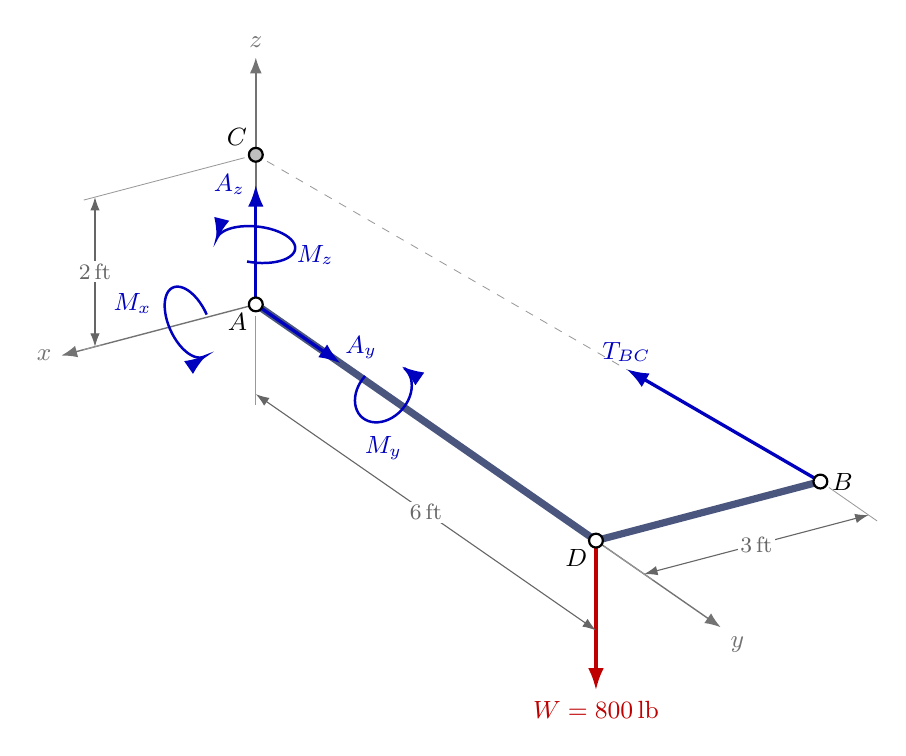
\begin{tikzpicture}[x={(-0.95cm,-0.25cm)}, y={(0.72cm,-0.5cm)}, z={(0cm,0.95cm)}, font=\small]
  \draw[axis] (0,0,0) -- (2.6,0,0) node[left]{$x$};
  \draw[axis] (0,0,0) -- (0,8.2,0) node[below right]{$y$};
  \draw[axis] (0,0,0) -- (0,0,3.3) node[above]{$z$};
  % member
  \draw[member] (0,0,0) -- (0,6,0) -- (-3,6,0);
  % cable stub (cut) and its force on B
  \draw[ext, dashed] (-3,6,0) -- (0,0,2);
  \draw[rxn] (-3,6,0) -- (-1.97,3.94,0.69) node[above, inner sep=2pt]{$T_{BC}$};
  % weight
  \draw[load] (0,6,-0.05) -- (0,6,-2.0) node[below]{$W=\SI{800}{lb}$};
  % reactions at A
  \draw[rxn] (0,0,0) -- (0,1.5,0) node[above right, inner sep=1pt]{$A_y$};
  \draw[rxn] (0,0,0) -- (0,0,1.6) node[left]{$A_z$};
  % couple moments as curl arrows (right-hand rule)
  \draw[rxn, line width=0.9pt, domain=40:320, samples=40] plot ({0.9},{0.42*cos(\x)},{0.42*sin(\x)});
  \node[blue!75!black] at (1.65,0,0.45) {$M_x$};
  \draw[rxn, line width=0.9pt, domain=40:320, samples=40] plot ({0.38*sin(\x)},{2.25},{0.38*cos(\x)});
  \node[blue!75!black, anchor=north] at (0,2.25,-0.45) {$M_y$};
  \draw[rxn, line width=0.9pt, domain=40:320, samples=40] plot ({0.42*cos(\x)},{0.42*sin(\x)},{0.8});
  \node[blue!75!black, anchor=west] at (0,0.55,0.95) {$M_z$};
  % points
  \node[pin] at (0,0,0) {}; \node[anchor=north east, inner sep=3pt] at (0,0,0) {$A$};
  \node[pin] at (0,6,0) {}; \node[anchor=north east, inner sep=3pt] at (0,6,0) {$D$};
  \node[pin] at (-3,6,0) {}; \node[anchor=west, inner sep=4pt] at (-3,6,0) {$B$};
  \node[pin, fill=black!25] at (0,0,2) {}; \node[anchor=south east, inner sep=3pt] at (0,0,2) {$C$};
  % dimensions
  \draw[ext] (0.15,0,2) -- (2.3,0,2); \draw[ext] (2.05,0,0) -- (2.3,0,0);
  \draw[dim] (2.15,0,0) -- node[dl]{\SI{2}{ft}} (2.15,0,2);
  \draw[ext] (0,0,-0.15) -- (0,0,-1.35);
  \draw[dim] (0,0,-1.2) -- node[dl]{\SI{6}{ft}} (0,6,-1.2);
  \draw[ext] (0,6.15,0) -- (0,7.0,0); \draw[ext] (-3,6.15,0) -- (-3,7.0,0);
  \draw[dim] (0,6.85,0) -- node[dl]{\SI{3}{ft}} (-3,6.85,0);
\end{tikzpicture}}
\end{sketchframe}

\textbf{Equations \& Solution:}\\
Because the rod fits loosely, the joint can slide along it, so $A_x=0$. The square cross-section still prevents rotation about all three axes, so $A$ also has couple moments $M_x$, $M_y$, and $M_z$.

The coordinates (in ft) are $A(0,0,0)$, $D(0,6,0)$, $B(-3,6,0)$, and $C(0,0,2)$. The cable runs along $\overrightarrow{BC}=(3,-6,2)$, which has a length of \SI{7}{\ft}.
\[
\mathbf T_{BC}=T_{BC}\left(\tfrac37,\,-\tfrac67,\,\tfrac27\right),\qquad \mathbf W=(0,0,-800)\ \si{\lb}\ \text{at } D
\]
\begin{align*}
\textstyle\sum F_x&:\ \tfrac37T_{BC}=0 &&\Rightarrow T_{BC}=0\\
\textstyle\sum F_y&:\ A_y-\tfrac67T_{BC}=0 &&\Rightarrow A_y=0\\
\textstyle\sum F_z&:\ A_z+\tfrac27T_{BC}-800=0 &&\Rightarrow A_z=\SI{800}{\lb}
\end{align*}
The cable is the only force on the member with an $x$-component, so its tension has to be zero.

With $T_{BC}=0$, the weight is the only force with a moment about $A$: $\mathbf r_{AD}\times\mathbf W=(0,6,0)\times(0,0,-800)=(-4800,0,0)$ lb$\cdot$ft.
\begin{align*}
\textstyle\sum M_x&:\ M_x-4800=0 &&\Rightarrow M_x=\SI{4800}{\lb\cdot\ft}\\
\textstyle\sum M_y&:\ M_y=0, \qquad \textstyle\sum M_z:\ M_z=0
\end{align*}

\begin{finalanswer}
$A_y=0$, \quad $A_z=\SI{800}{\lb}$, \quad $M_x=\SI{4.80e3}{\lb\cdot\ft}$, \quad $M_y=M_z=0$, \quad $T_{BC}=0$
\end{finalanswer}

% =========================================================
% PROBLEM 3
% =========================================================
\problemstart{3}{The truss has a pin at $A$ and a roller at $C$ on a surface inclined at $\theta=30^\circ$. Find the force in each member and state whether it is in tension or compression.}

\begin{sketchframe}
\scalebox{1.05}{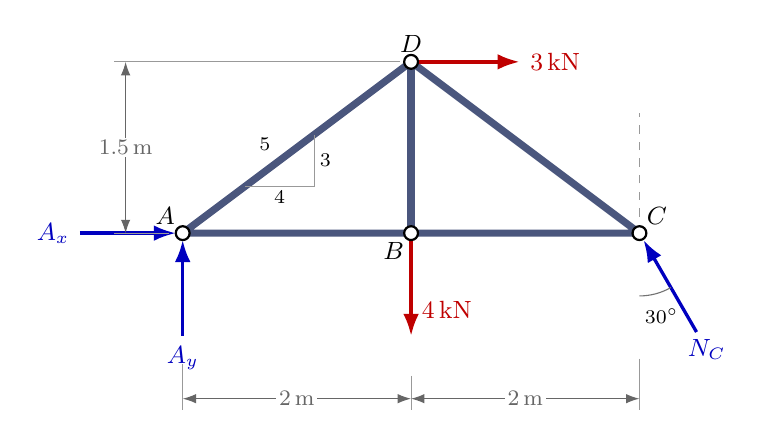
\begin{tikzpicture}[scale=1.45, font=\small]
  \coordinate (A) at (0,0); \coordinate (B) at (2,0); \coordinate (C) at (4,0); \coordinate (D) at (2,1.5);
  \draw[member] (A) -- (B) -- (C) -- (D) -- cycle; \draw[member] (B) -- (D);
  % slope triangle on AD
  \draw[ext] (0.55,0.4125) -- (1.15,0.4125) -- (1.15,0.8625);
  \node[font=\scriptsize] at (0.85,0.31) {4}; \node[font=\scriptsize] at (1.25,0.64) {3};
  \node[font=\scriptsize] at (0.72,0.78) {5};
  % loads
  \draw[load] (B) -- ++(0,-0.9) node[right, pos=0.75]{\SI{4}{kN}};
  \draw[load] (D) -- ++(0.95,0) node[right]{\SI{3}{kN}};
  % reactions
  \draw[rxn] (-0.9,0) node[left]{$A_x$} -- ($(A)+(-0.06,0)$);
  \draw[rxn] (0,-0.9) node[below]{$A_y$} -- ($(A)+(0,-0.06)$);
  % N_C normal to 30 deg incline: direction 120 deg
  \draw[ext, dashed] (C) -- ++(0,1.05);
  \draw[rxn] ($(C)+(-60:1.0)$) -- ($(C)+(-60:0.07)$);
  \node[blue!75!black] at ($(C)+(-60:1.18)$) {$N_C$};
  \draw[black!55, line width=0.4pt] ($(C)+(-90:0.55)$) arc (-90:-60:0.55);
  \node[font=\scriptsize] at ($(C)+(-75:0.75)$) {$30^\circ$};
  \foreach \p/\n/\a in {A/A/135, B/B/225, C/C/45, D/D/90} { \node[pin] at (\p) {}; \node[anchor=\a+180, inner sep=3pt] at (\p) {$\n$}; }
  % dims
  \draw[ext] (0,-1.15) -- (0,-1.55); \draw[ext] (2,-1.25) -- (2,-1.55); \draw[ext] (4,-1.1) -- (4,-1.55);
  \draw[dim] (0,-1.45) -- node[dl]{\SI{2}{m}} (2,-1.45);
  \draw[dim] (2,-1.45) -- node[dl]{\SI{2}{m}} (4,-1.45);
  \draw[ext] (1.9,1.5) -- (-0.6,1.5); \draw[ext] (-0.12,0) -- (-0.6,0);
  \draw[dim] (-0.5,0) -- node[dl]{\SI{1.5}{m}} (-0.5,1.5);
\end{tikzpicture}}

\vspace{4mm}
\scalebox{0.86}{\jfbd{Joint A}{\rin{180}{\SI{1.20}{kN}}\rin{270}{\SI{0.875}{kN}}\mT{0}{$F_{AB}$}\mT{36.87}{$F_{AD}$}}
\jfbd{Joint B}{\mT{180}{$F_{AB}$}\mT{0}{$F_{BC}$}\mT{90}{$F_{BD}$}\fout{270}{\SI{4}{kN}}}
\jfbd{Joint C}{\mT{180}{$F_{BC}$}\mT{143.13}{$F_{CD}$}\rin{300}{\SI{3.61}{kN}}}}
\end{sketchframe}

\textbf{Equations \& Solution:}\\
The roller reaction $N_C$ acts normal to the incline, which puts it $30^\circ$ from vertical. Solving for the support reactions:
\begin{align*}
\textstyle\sum M_A&:\ N_C\cos30^\circ(4)-4(2)-3(1.5)=0 &&\Rightarrow N_C=\SI{3.608}{\kN}\\
\textstyle\sum F_x&:\ A_x+3-N_C\sin30^\circ=0 &&\Rightarrow A_x=\SI{-1.196}{\kN}\\
\textstyle\sum F_y&:\ A_y-4+N_C\cos30^\circ=0 &&\Rightarrow A_y=\SI{0.875}{\kN}
\end{align*}
Members $AD$ and $CD$ form 3-4-5 triangles, so their direction cosines are 0.8 and 0.6. Working through the joints:
\begin{align*}
A:\ \textstyle\sum F_y&=0.875+0.6F_{AD}=0 &&\Rightarrow F_{AD}=\SI{-1.458}{\kN}\\
\textstyle\sum F_x&=-1.196+F_{AB}+0.8F_{AD}=0 &&\Rightarrow F_{AB}=\SI{2.363}{\kN}\\
B:\ \textstyle\sum F_x&=F_{BC}-F_{AB}=0 &&\Rightarrow F_{BC}=\SI{2.363}{\kN}\\
\textstyle\sum F_y&=F_{BD}-4=0 &&\Rightarrow F_{BD}=\SI{4.000}{\kN}\\
C:\ \textstyle\sum F_y&=3.125+0.6F_{CD}=0 &&\Rightarrow F_{CD}=\SI{-5.208}{\kN}
\end{align*}

\begin{finalanswer}
$F_{AB}=\SI{2.36}{\kN}$ (T), \ $F_{AD}=\SI{1.46}{\kN}$ (C), \ $F_{BC}=\SI{2.36}{\kN}$ (T), \ $F_{BD}=\SI{4.00}{\kN}$ (T), \ $F_{CD}=\SI{5.21}{\kN}$ (C)
\end{finalanswer}

% =========================================================
% PROBLEM 4
% =========================================================
\problemstart{4}{Members $AB$ and $BC$ can each support a maximum compressive force of \SI{800}{\lb}, and members $AD$, $DC$, and $BD$ can each support a maximum tensile force of \SI{2000}{\lb}. With $a=\SI{6}{\ft}$, find the greatest load $P$ the truss can carry.}

\begin{sketchframe}
\scalebox{0.8}{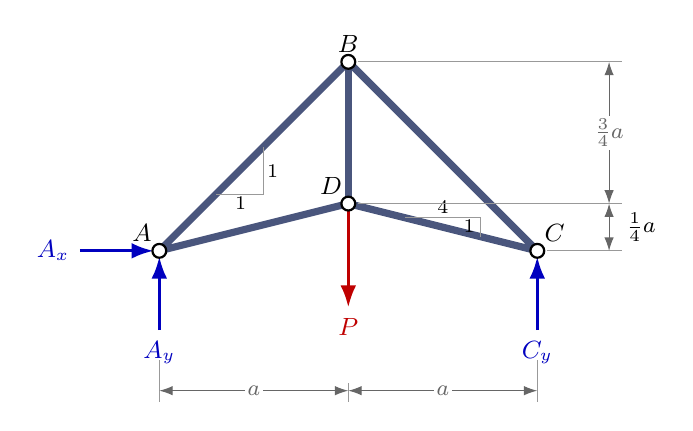
\begin{tikzpicture}[scale=2.4, font=\small]
  \coordinate (A) at (0,0); \coordinate (B) at (1,1); \coordinate (C) at (2,0); \coordinate (D) at (1,0.25);
  \draw[member] (A) -- (B) -- (C) -- (D) -- cycle; \draw[member] (B) -- (D);
  % slope marks
  \draw[ext] (0.3,0.3) -- (0.55,0.3) -- (0.55,0.55); \node[font=\scriptsize] at (0.43,0.25) {1}; \node[font=\scriptsize] at (0.6,0.42) {1};
  \draw[ext] (1.3,0.175) -- (1.7,0.175) -- (1.7,0.075); \node[font=\scriptsize] at (1.5,0.23) {4}; \node[font=\scriptsize] at (1.64,0.13) {1};
  \draw[load] (D) -- ++(0,-0.55) node[below]{$P$};
  \draw[rxn] (-0.42,0) node[left]{$A_x$} -- (-0.03,0);
  \draw[rxn] (0,-0.42) node[below]{$A_y$} -- (0,-0.03);
  \draw[rxn] (2,-0.42) node[below]{$C_y$} -- (2,-0.03);
  \foreach \p/\n/\a in {A/A/135, B/B/90, C/C/45, D/D/135} { \node[pin] at (\p) {}; \node[anchor=\a+180, inner sep=3pt] at (\p) {$\n$}; }
  \draw[ext] (0,-0.58) -- (0,-0.8); \draw[ext] (2,-0.58) -- (2,-0.8); \draw[ext] (1,-0.7) -- (1,-0.8);
  \draw[dim] (0,-0.74) -- node[dl]{$a$} (1,-0.74); \draw[dim] (1,-0.74) -- node[dl]{$a$} (2,-0.74);
  \draw[ext] (1.05,1) -- (2.45,1); \draw[ext] (1.05,0.25) -- (2.45,0.25); \draw[ext] (2.05,0) -- (2.45,0);
  \draw[dim] (2.38,0.25) -- node[dl]{$\tfrac34a$} (2.38,1);
  \draw[dim] (2.38,0) -- (2.38,0.25); \node[font=\footnotesize, anchor=west] at (2.42,0.125) {$\tfrac14a$};
\end{tikzpicture}}

\vspace{2mm}
\scalebox{0.85}{\jfbd{Joint A}{\rin{270}{$P/2$}\mT{45}{$F_{AB}$}\mT{14.04}{$F_{AD}$}}\hspace{6mm}
\jfbd{Joint D}{\mT{194.04}{$F_{AD}$}\mT{345.96}{$F_{DC}$}\mT{90}{$F_{BD}$}\fout{270}{$P$}}}
\end{sketchframe}

\textbf{Equations \& Solution:}\\
Member $AB$ is at $45^\circ$ and member $AD$ is at $\varphi=\tan^{-1}(1/4)=14.04^\circ$. The truss and load are symmetric, so each support carries half the load ($A_y=C_y=P/2$), and $A_x=0$ because there are no horizontal loads.
\begin{align*}
A:\ \textstyle\sum F_x&=F_{AB}\cos45^\circ+F_{AD}\cos\varphi=0 &&\Rightarrow F_{AD}=-0.7289F_{AB}\\
\textstyle\sum F_y&=\tfrac P2+F_{AB}\sin45^\circ+F_{AD}\sin\varphi=0 &&\Rightarrow F_{AB}=-0.9428P,\quad F_{AD}=0.6872P\\
D:\ \textstyle\sum F_y&=F_{BD}-2F_{AD}\sin\varphi-P=0 &&\Rightarrow F_{BD}=1.333P
\end{align*}
By symmetry, $F_{BC}=F_{AB}$ and $F_{DC}=F_{AD}$. Setting each member force equal to its limit gives the largest $P$ that member allows:
\begin{center}
\begin{tabular}{lccc}
\toprule
\textbf{Member} & \textbf{Force} & \textbf{Limit} & \textbf{Max.\ $P$} \\
\midrule
$AB$, $BC$ (C) & $0.9428P$ & \SI{800}{\lb} & \SI{848.5}{\lb}\\
$AD$, $DC$ (T) & $0.6872P$ & \SI{2000}{\lb} & \SI{2910}{\lb}\\
$BD$ (T) & $1.333P$ & \SI{2000}{\lb} & \SI{1500}{\lb}\\
\bottomrule
\end{tabular}
\end{center}
The smallest of these is \SI{848.5}{\lb}, from members $AB$ and $BC$, so they reach their limit first. With $P$ rounded down to \SI{848}{\lb}, the force in $AB$ and $BC$ is $0.9428(848)=\SI{799.5}{\lb}$, which stays under the \SI{800}{\lb} limit.

\begin{finalanswer}
$P_{\max}=\SI{848}{\lb}$
\end{finalanswer}

% =========================================================
% PROBLEM 5
% =========================================================
\problemstart{5}{The maximum allowable tensile force in any member is \SI{5}{\kN}, and the maximum allowable compressive force is \SI{3}{\kN}. With $d=\SI{2}{m}$, find the maximum load $P$ that can be applied to the truss.}

\begin{sketchframe}
\scalebox{1.25}{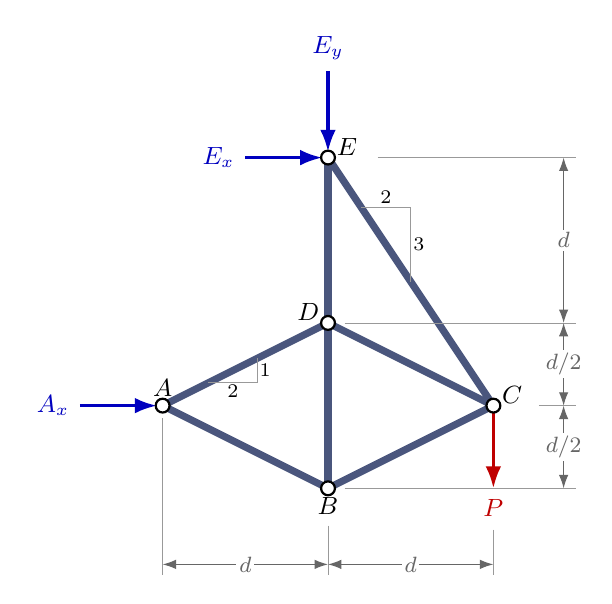
\begin{tikzpicture}[scale=1.05, font=\small]
  % d = 2 m drawn 1 unit = 1 m
  \coordinate (A) at (0,1); \coordinate (B) at (2,0); \coordinate (D) at (2,2); \coordinate (C) at (4,1); \coordinate (E) at (2,4);
  \draw[member] (A) -- (D) -- (C) -- (B) -- cycle; \draw[member] (E) -- (B); \draw[member] (E) -- (C);
  % slope triangles
  \draw[ext] (0.55,1.275) -- (1.15,1.275) -- (1.15,1.575); \node[font=\scriptsize] at (0.85,1.17) {2}; \node[font=\scriptsize] at (1.24,1.43) {1};
  \draw[ext] (3.0,2.5) -- (3.0,3.4) -- (2.4,3.4); \node[font=\scriptsize] at (3.1,2.95) {3}; \node[font=\scriptsize] at (2.7,3.52) {2};
  \draw[load] (C) -- ++(0,-1.0) node[below]{$P$};
  \draw[rxn] (-1.0,1) node[left]{$A_x$} -- (-0.07,1);
  \draw[rxn] (1.0,4) node[left]{$E_x$} -- (1.93,4);
  \draw[rxn] (2,5.05) node[above]{$E_y$} -- (2,4.07);
  \foreach \p/\n/\a in {A/A/90, B/B/270, C/C/30, D/D/150, E/E/30} { \node[pin] at (\p) {}; \node[anchor=\a+180, inner sep=3pt] at (\p) {$\n$}; }
  % dims
  \draw[ext] (0,0.85) -- (0,-1.05); \draw[ext] (2,-0.45) -- (2,-1.05); \draw[ext] (4,-0.5) -- (4,-1.05);
  \draw[dim] (0,-0.92) -- node[dl]{$d$} (2,-0.92); \draw[dim] (2,-0.92) -- node[dl]{$d$} (4,-0.92);
  \draw[ext] (2.6,4) -- (5.0,4); \draw[ext] (2.2,2) -- (5.0,2); \draw[ext] (4.55,1) -- (5.0,1); \draw[ext] (2.2,0) -- (5.0,0);
  \draw[dim] (4.85,2) -- node[dl]{$d$} (4.85,4);
  \draw[dim] (4.85,1) -- node[dl]{$d/2$} (4.85,2);
  \draw[dim] (4.85,0) -- node[dl]{$d/2$} (4.85,1);
\end{tikzpicture}}

\vspace{4mm}
\scalebox{0.86}{\jfbd{Joint A}{\rin{180}{$A_x$}\mT{26.57}{$F_{AD}$}\mT{-26.57}{$F_{AB}$}}
\jfbd{Joint B}{\mT{153.43}{$F_{AB}$}\mT{26.57}{$F_{BC}$}\mT{90}{$F_{BD}$}}
\jfbd{Joint D}{\mT{206.57}{$F_{AD}$}\mT{-26.57}{$F_{DC}$}\mT{270}{$F_{BD}$}\mT{90}{$F_{DE}$}}
\jfbd{Joint C}{\mT{123.69}{$F_{CE}$}\mT{153.43}{$F_{CD}$}\mT{206.57}{$F_{BC}$}\fout{270}{$P$}}}
\end{sketchframe}

\textbf{Equations \& Solution:}\\
$E$ is a pin, so it has reactions $E_x$ and $E_y$. $A$ is a roller against the wall, so it can only push horizontally, which means $A_y=0$.

Members $AD$, $AB$, $DC$, and $BC$ have a 1:2 slope (direction cosines $\tfrac{2}{\sqrt5}$ and $\tfrac{1}{\sqrt5}$), and $EC$ has a 3:2 slope (direction cosines $\tfrac{2}{\sqrt{13}}$ and $\tfrac{3}{\sqrt{13}}$).

Working through joints $A$, $B$, and $D$ shows that $DE$ is a zero-force member:
\begin{align*}
A:\ \textstyle\sum F_y&=\tfrac{1}{\sqrt5}(F_{AD}-F_{AB})=0 &&\Rightarrow F_{AD}=F_{AB}\\
B:\ \textstyle\sum F_x&=\tfrac{2}{\sqrt5}(F_{BC}-F_{AB})=0 &&\Rightarrow F_{BC}=F_{AB}\\
\textstyle\sum F_y&=F_{BD}+\tfrac{1}{\sqrt5}(F_{AB}+F_{BC})=0 &&\Rightarrow F_{BD}=-\tfrac{2}{\sqrt5}F_{AB}\\
D:\ \textstyle\sum F_x&=\tfrac{2}{\sqrt5}(F_{DC}-F_{AD})=0 &&\Rightarrow F_{DC}=F_{AD}=F_{AB}\\
\textstyle\sum F_y&=F_{DE}-F_{BD}-\tfrac{1}{\sqrt5}(F_{AD}+F_{DC})=0 &&\Rightarrow F_{DE}=-\tfrac{2}{\sqrt5}F_{AB}+\tfrac{2}{\sqrt5}F_{AB}=0
\end{align*}
Everything is now in terms of $F_{AB}$, so joint $C$ only has two unknowns, $F_{CE}$ and $F_{AB}$:
\begin{align*}
\textstyle\sum F_y&=\tfrac{3}{\sqrt{13}}F_{CE}+\tfrac{1}{\sqrt5}(F_{CD}-F_{BC})-P=0 &&\Rightarrow F_{CE}=\tfrac{\sqrt{13}}{3}P=1.202P\\
\textstyle\sum F_x&=-\tfrac{2}{\sqrt{13}}F_{CE}-\tfrac{2}{\sqrt5}(F_{CD}+F_{BC})=0 &&\Rightarrow F_{AB}=-0.3727P
\end{align*}
This gives $F_{AD}=F_{AB}=F_{DC}=F_{BC}=0.3727P$ (C), $F_{BD}=0.3333P$ (T), $F_{CE}=1.202P$ (T), and $F_{DE}=0$. Setting each member force equal to its limit:
\begin{center}
\begin{tabular}{lccc}
\toprule
\textbf{Member} & \textbf{Force} & \textbf{Limit} & \textbf{Max.\ $P$} \\
\midrule
$CE$ (T) & $1.202P$ & \SI{5}{\kN} & \SI{4.160}{\kN}\\
$BD$ (T) & $0.3333P$ & \SI{5}{\kN} & \SI{15.0}{\kN}\\
$AD$, $AB$, $DC$, $BC$ (C) & $0.3727P$ & \SI{3}{\kN} & \SI{8.05}{\kN}\\
\bottomrule
\end{tabular}
\end{center}

Member $CE$ reaches its \SI{5}{\kN} tension limit first, so it sets the maximum load.

\begin{finalanswer}
$P_{\max}=\SI{4.16}{\kN}$
\end{finalanswer}

% =========================================================
% PROBLEM 6
% =========================================================
\problemstart{6}{Determine the forces in members $EF$, $CF$, and $BC$ and state whether they are in tension or compression.}

\begin{sketchframe}
\scalebox{1.0}{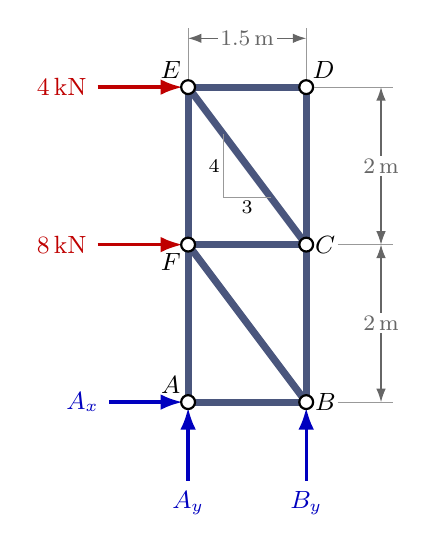
\begin{tikzpicture}[scale=1.0, font=\small]
  \coordinate (A) at (0,0); \coordinate (B) at (1.5,0); \coordinate (C) at (1.5,2); \coordinate (D) at (1.5,4); \coordinate (E) at (0,4); \coordinate (F) at (0,2);
  \draw[member] (A) -- (B) -- (D) -- (E) -- cycle; \draw[member] (F) -- (C); \draw[member] (E) -- (C); \draw[member] (F) -- (B);
  % slope triangle on EC
  \draw[ext] (0.45,3.4) -- (0.45,2.6) -- (1.05,2.6); \node[font=\scriptsize] at (0.33,3.0) {4}; \node[font=\scriptsize] at (0.75,2.47) {3};
  \draw[load] (-1.15,4) node[left]{\SI{4}{kN}} -- (-0.07,4);
  \draw[load] (-1.15,2) node[left]{\SI{8}{kN}} -- (-0.07,2);
  \draw[rxn] (-1.0,0) node[left]{$A_x$} -- (-0.07,0);
  \draw[rxn] (0,-1.0) node[below]{$A_y$} -- (0,-0.07);
  \draw[rxn] (1.5,-1.0) node[below]{$B_y$} -- (1.5,-0.07);
  \foreach \p/\n/\a in {A/A/135, B/B/0, C/C/0, D/D/45, E/E/135, F/F/225} { \node[pin] at (\p) {}; \node[anchor=\a+180, inner sep=3pt] at (\p) {$\n$}; }
  \draw[ext] (0,4.1) -- (0,4.75); \draw[ext] (1.5,4.1) -- (1.5,4.75);
  \draw[dim] (0,4.62) -- node[dl]{\SI{1.5}{m}} (1.5,4.62);
  \draw[ext] (1.6,4) -- (2.6,4); \draw[ext] (1.9,2) -- (2.6,2); \draw[ext] (1.9,0) -- (2.6,0);
  \draw[dim] (2.45,2) -- node[dl]{\SI{2}{m}} (2.45,4); \draw[dim] (2.45,0) -- node[dl]{\SI{2}{m}} (2.45,2);
\end{tikzpicture}}

\vspace{4mm}
\jfbd{Joint D}{\mT{180}{$F_{DE}$}\mT{270}{$F_{DC}$}}
\jfbd{Joint E}{\fin{180}{\SI{4}{kN}}\mT{0}{$F_{ED}$}\mT{270}{$F_{EF}$}\mT{-53.13}{$F_{EC}$}}
\jfbd{Joint C}{\mT{90}{$F_{CD}$}\mT{126.87}{$F_{CE}$}\mT{180}{$F_{CF}$}\mT{270}{$F_{BC}$}}
\end{sketchframe}

\textbf{Equations \& Solution:}\\
Joint $D$ has no load and only two members, and they are not collinear, so $DE$ and $DC$ are both zero-force members. Starting at joint $E$ means the support reactions are not needed.

Member $EC$ spans \SI{1.5}{m} horizontally and \SI{2}{m} vertically, a 3-4-5 triangle, so its direction from $E$ to $C$ is $(0.6,\,-0.8)$.
\begin{align*}
E:\ \textstyle\sum F_x&=4+0.6F_{EC}=0 &&\Rightarrow F_{EC}=\SI{-6.667}{\kN}\\
\textstyle\sum F_y&=-F_{EF}-0.8F_{EC}=0 &&\Rightarrow F_{EF}=\SI{5.333}{\kN}\\
C:\ \textstyle\sum F_x&=-0.6F_{CE}-F_{CF}=0 &&\Rightarrow F_{CF}=\SI{4.000}{\kN}\\
\textstyle\sum F_y&=0.8F_{CE}-F_{BC}=0 &&\Rightarrow F_{BC}=\SI{-5.333}{\kN}
\end{align*}

\begin{finalanswer}
$F_{EF}=\SI{5.33}{\kN}$ (T), \quad $F_{CF}=\SI{4.00}{\kN}$ (T), \quad $F_{BC}=\SI{5.33}{\kN}$ (C)
\end{finalanswer}

% =========================================================
% PROBLEM 7
% =========================================================
\problemstart{7}{The truss has a pin at $A$ and a roller at $G$. Determine the forces in members $BF$, $BG$, and $AB$ and state whether they are in tension or compression.}

\begin{sketchframe}
\scalebox{0.85}{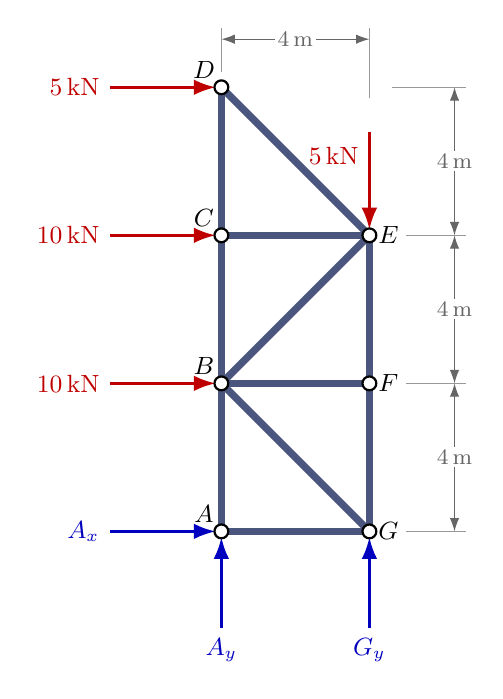
\begin{tikzpicture}[scale=0.47, font=\small]
  \coordinate (A) at (0,0); \coordinate (B) at (0,4); \coordinate (C) at (0,8); \coordinate (D) at (0,12);
  \coordinate (G) at (4,0); \coordinate (F) at (4,4); \coordinate (E) at (4,8);
  \draw[member] (A) -- (D); \draw[member] (G) -- (E);
  \draw[member] (A) -- (G); \draw[member] (B) -- (F); \draw[member] (C) -- (E);
  \draw[member] (D) -- (E); \draw[member] (B) -- (E); \draw[member] (B) -- (G);
  \draw[load] (-3.0,12) -- (-0.15,12) node[pos=0.0, left]{\SI{5}{kN}};
  \draw[load] (-3.0,8) -- (-0.15,8) node[pos=0.0, left]{\SI{10}{kN}};
  \draw[load] (-3.0,4) -- (-0.15,4) node[pos=0.0, left]{\SI{10}{kN}};
  \draw[load] (4,10.8) -- (4,8.15) node[pos=0.25, left]{\SI{5}{kN}};
  \draw[rxn] (-3.0,0) node[left]{$A_x$} -- (-0.15,0);
  \draw[rxn] (0,-2.6) node[below]{$A_y$} -- (0,-0.15);
  \draw[rxn] (4,-2.6) node[below]{$G_y$} -- (4,-0.15);
  \foreach \p/\n/\a in {A/A/135, B/B/135, C/C/135, D/D/135, E/E/0, F/F/0, G/G/0} { \node[pin] at (\p) {}; \node[anchor=\a+180, inner sep=3pt] at (\p) {$\n$}; }
  \foreach \y in {0,4,8} \draw[ext] (5.0,\y) -- (6.6,\y);
  \draw[ext] (4.6,12) -- (6.6,12);
  \draw[dim] (6.3,0) -- node[dl]{\SI{4}{m}} (6.3,4); \draw[dim] (6.3,4) -- node[dl]{\SI{4}{m}} (6.3,8); \draw[dim] (6.3,8) -- node[dl]{\SI{4}{m}} (6.3,12);
  \draw[ext] (0,12.4) -- (0,13.6); \draw[ext] (4,11.7) -- (4,13.6);
  
  \draw[dim] (0,13.3) -- node[dl]{\SI{4}{m}} (4,13.3);
\end{tikzpicture}}

\vspace{4mm}
\jfbd{Joint A}{\rout{180}{\SI{25}{kN}}\rout{270}{\SI{45}{kN}}\mT{90}{$F_{AB}$}\mT{0}{$F_{AG}$}}
\jfbd{Joint F}{\mT{180}{$F_{BF}$}\mT{90}{$F_{EF}$}\mT{270}{$F_{FG}$}}
\jfbd{Joint G}{\rin{270}{\SI{50}{kN}}\mT{180}{$F_{AG}$}\mT{90}{$F_{FG}$}\mT{135}{$F_{BG}$}\jang{135}{180}{$45^\circ$}}
\end{sketchframe}

\textbf{Equations \& Solution:}\\
Solving for the support reactions:
\begin{align*}
\textstyle\sum M_A&:\ 4G_y-5(12)-10(8)-10(4)-5(4)=0 &&\Rightarrow G_y=\SI{50.0}{\kN}\\
\textstyle\sum F_x&:\ A_x+25=0 &&\Rightarrow A_x=\SI{-25.0}{\kN}\\
\textstyle\sum F_y&:\ A_y+50-5=0 &&\Rightarrow A_y=\SI{-45.0}{\kN}
\end{align*}
At joint $F$, members $EF$ and $FG$ are collinear and there is no external load, so $BF$ is a zero-force member and $F_{BF}=0$. The other two forces come from joints $A$ and $G$:
\begin{align*}
A:\ \textstyle\sum F_y&=-45+F_{AB}=0 &&\Rightarrow F_{AB}=\SI{45.0}{\kN}\\
\textstyle\sum F_x&=-25+F_{AG}=0 &&\Rightarrow F_{AG}=\SI{25.0}{\kN}\\
G:\ \textstyle\sum F_x&=-F_{AG}-F_{BG}\cos45^\circ=0 &&\Rightarrow F_{BG}=\SI{-35.36}{\kN}
\end{align*}

\begin{finalanswer}
$F_{AB}=\SI{45.0}{\kN}$ (T), \quad $F_{BF}=0$, \quad $F_{BG}=\SI{35.4}{\kN}$ (C)
\end{finalanswer}

% =========================================================
% PROBLEM 8
% =========================================================
\problemstart{8}{The space truss is supported by ball-and-socket joints at $A$, $B$, $C$, and $D$. Find the force in each member and state whether it is in tension or compression.}

\begin{sketchframe}
\scalebox{1.15}{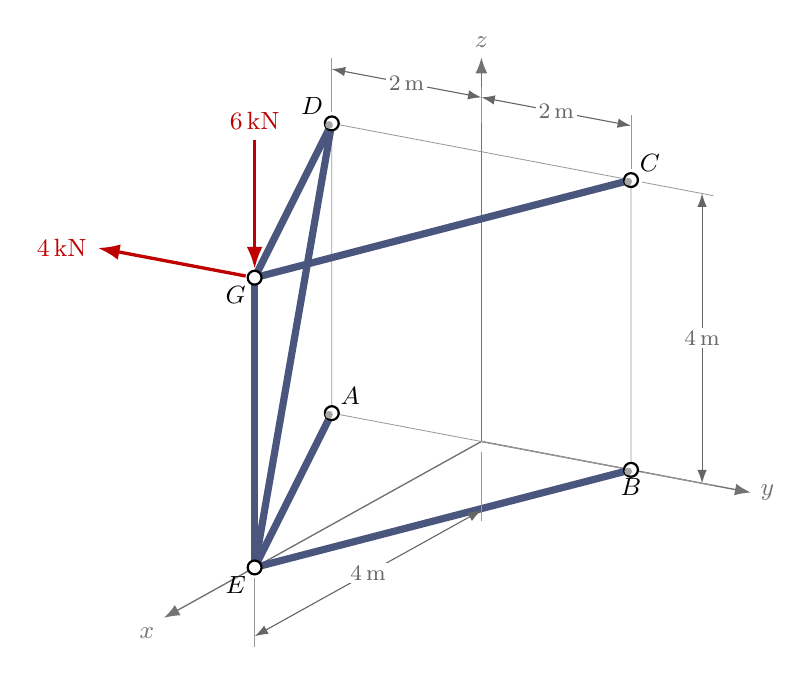
\begin{tikzpicture}[x={(-0.72cm,-0.4cm)}, y={(0.95cm,-0.18cm)}, z={(0cm,0.92cm)}, font=\small]
  \draw[axis] (0,0,0) -- (5.6,0,0) node[below left]{$x$};
  \draw[axis] (0,0,0) -- (0,3.6,0) node[right]{$y$};
  \draw[axis] (0,0,0) -- (0,0,5.3) node[above]{$z$};
  % support plane outline
  \draw[ext] (0,-2,0) -- (0,-2,4) -- (0,2,4) -- (0,2,0) -- cycle;
  % members
  \draw[member] (4,0,0) -- (4,0,4);
  \draw[member] (4,0,4) -- (0,-2,4);
  \draw[member] (4,0,4) -- (0,2,4);
  \draw[member] (4,0,0) -- (0,-2,4);
  \draw[member] (4,0,0) -- (0,-2,0);
  \draw[member] (4,0,0) -- (0,2,0);
  % loads at G
  \draw[load] (4,0,5.9) -- (4,0,4.12) node[pos=0.0, above]{\SI{6}{kN}};
  \draw[load] (4,0,4) ++(0,-0.12,0) -- (4,-2.1,4) node[left]{\SI{4}{kN}};
  % joints
  \foreach \p/\n/\a in {{(0,-2,0)}/A/south west, {(0,2,0)}/B/north, {(0,2,4)}/C/south west, {(0,-2,4)}/D/south east, {(4,0,0)}/E/north east, {(4,0,4)}/G/north east} {
    \node[pin] at \p {}; \node[anchor=\a, inner sep=3pt] at \p {$\n$};
  }
  \foreach \p in {{(0,-2,0)},{(0,2,0)},{(0,2,4)},{(0,-2,4)}} \fill[black!35] \p ++(0.05,0,0) circle (1.4pt);
  % dimensions
  \draw[ext] (0,-2,4.15) -- (0,-2,4.9); \draw[ext] (0,0,4.4) -- (0,0,4.9); \draw[ext] (0,2,4.15) -- (0,2,4.9);
  \draw[dim] (0,-2,4.75) -- node[dl]{\SI{2}{m}} (0,0,4.75);
  \draw[dim] (0,0,4.75) -- node[dl]{\SI{2}{m}} (0,2,4.75);
  \draw[ext] (0,2.15,0) -- (0,3.1,0); \draw[ext] (0,2.15,4) -- (0,3.1,4);
  \draw[dim] (0,2.95,0) -- node[dl]{\SI{4}{m}} (0,2.95,4);
  \draw[ext] (0,0,-0.15) -- (0,0,-1.1); \draw[ext] (4,0,-0.15) -- (4,0,-1.1);
  \draw[dim] (0,0,-0.95) -- node[dl]{\SI{4}{m}} (4,0,-0.95);
\end{tikzpicture}}

\vspace{4mm}
\scalebox{0.95}{% rotated view for the joint FBDs so the members at E separate
\begin{tabular}{@{}c@{\hspace{10mm}}c@{}}
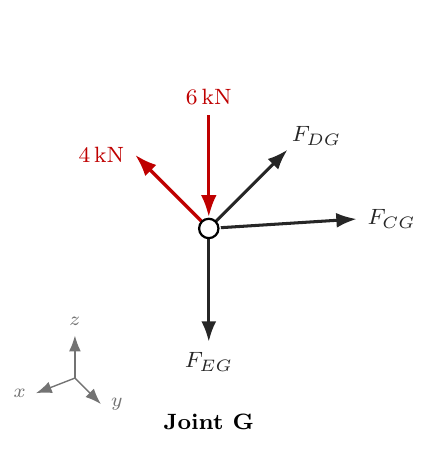
\begin{tikzpicture}[x={(-0.9cm,-0.35cm)}, y={(0.55cm,-0.55cm)}, z={(0cm,0.9cm)}, font=\footnotesize, baseline=(cap.base)]
  \path[use as bounding box] (-2.3cm,-2.6cm) rectangle (2.45cm,2.55cm);
  \draw[mf] (0,0,-0.14) -- (0,0,-1.6) node[below]{$F_{EG}$};
  \draw[mf] (-0.13,0.065,0) -- (-1.6,0.8,0) node[right]{$F_{CG}$};
  \draw[mf] (-0.13,-0.065,0) -- (-1.6,-0.8,0) node[above right, inner sep=1pt]{$F_{DG}$};
  \draw[load] (0,0,1.6) -- (0,0,0.16) node[pos=0, above]{\SI{6}{kN}};
  \draw[load] (0,0.14,0) ++(0,-0.28,0) -- (0,-1.7,0) node[left]{\SI{4}{kN}};
  \node[pin, minimum size=7pt] at (0,0,0) {};
  \begin{scope}[shift={(-1.7cm,-1.9cm)}]
    \draw[axis] (0,0,0) -- (0.55,0,0) node[left, font=\scriptsize]{$x$};
    \draw[axis] (0,0,0) -- (0,0.6,0) node[right, font=\scriptsize]{$y$};
    \draw[axis] (0,0,0) -- (0,0,0.6) node[above, font=\scriptsize]{$z$};
  \end{scope}
  \node[font=\footnotesize\bfseries] (cap) at (0,-2.45cm) {Joint G};
\end{tikzpicture}
&
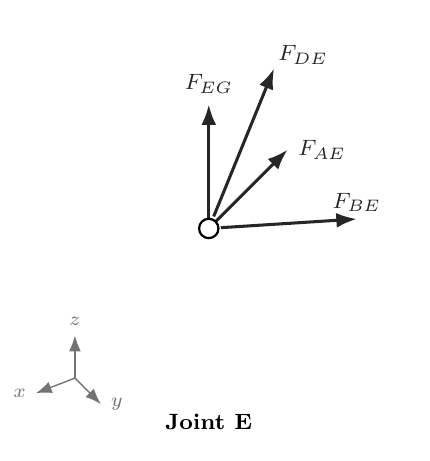
\begin{tikzpicture}[x={(-0.9cm,-0.35cm)}, y={(0.55cm,-0.55cm)}, z={(0cm,0.9cm)}, font=\footnotesize, baseline=(cap.base)]
  \path[use as bounding box] (-2.3cm,-2.6cm) rectangle (2.45cm,2.55cm);
  \draw[mf] (0,0,0.14) -- (0,0,1.75) node[above]{$F_{EG}$};
  \draw[mf] (-0.13,-0.065,0) -- (-1.6,-0.8,0) node[right]{$F_{AE}$};
  \draw[mf] (-0.13,0.065,0) -- (-1.6,0.8,0) node[above, inner sep=2pt]{$F_{BE}$};
  \draw[mf] (-0.1,-0.05,0.1) -- (-1.33,-0.67,1.33) node[above right, inner sep=1pt]{$F_{DE}$};
  \node[pin, minimum size=7pt] at (0,0,0) {};
  \begin{scope}[shift={(-1.7cm,-1.9cm)}]
    \draw[axis] (0,0,0) -- (0.55,0,0) node[left, font=\scriptsize]{$x$};
    \draw[axis] (0,0,0) -- (0,0.6,0) node[right, font=\scriptsize]{$y$};
    \draw[axis] (0,0,0) -- (0,0,0.6) node[above, font=\scriptsize]{$z$};
  \end{scope}
  \node[font=\footnotesize\bfseries] (cap) at (0,-2.45cm) {Joint E};
\end{tikzpicture}
\end{tabular}}
\end{sketchframe}

\clearpage
\textbf{Equations \& Solution:}\\
The coordinates (in m) are $A(0,-2,0)$, $B(0,2,0)$, $C(0,2,4)$, $D(0,-2,4)$, $E(4,0,0)$, and $G(4,0,4)$. The joint FBDs are drawn from a rotated view so the members at $E$ do not overlap. Joint $G$ only has three unknown member forces, so I solved it first and then moved to $E$.

\textbf{Joint $G$:} the unit vectors from $G$ toward $E$, $C$, and $D$ are $(0,0,-1)$, $(-0.8944,\,0.4472,\,0)$, and $(-0.8944,\,-0.4472,\,0)$. The applied load is $(0,-4,-6)$ kN.
\begin{align*}
\textstyle\sum F_x&=-0.8944(F_{CG}+F_{DG})=0 &&\Rightarrow F_{DG}=-F_{CG}\\
\textstyle\sum F_y&=0.4472(F_{CG}-F_{DG})-4=0 &&\Rightarrow F_{CG}=\SI{4.472}{\kN},\ F_{DG}=\SI{-4.472}{\kN}\\
\textstyle\sum F_z&=-F_{EG}-6=0 &&\Rightarrow F_{EG}=\SI{-6.00}{\kN}
\end{align*}
\textbf{Joint $E$:} the unit vectors from $E$ toward $A$, $B$, and $D$ are $(-0.8944,\,-0.4472,\,0)$, $(-0.8944,\,0.4472,\,0)$, and $(-0.6667,\,-0.3333,\,0.6667)$. There is no external load at $E$.
\begin{align*}
\textstyle\sum F_z&=F_{EG}+0.6667F_{DE}=0 &&\Rightarrow F_{DE}=\SI{9.00}{\kN}\\
\textstyle\sum F_x&=-0.8944(F_{AE}+F_{BE})-0.6667(9)=0 &&\Rightarrow F_{AE}+F_{BE}=-6.708\\
\textstyle\sum F_y&=0.4472(F_{BE}-F_{AE})-0.3333(9)=0 &&\Rightarrow F_{BE}-F_{AE}=6.708
\end{align*}
Solving the last two equations together gives $F_{BE}=0$ and $F_{AE}=\SI{-6.708}{\kN}$.

\begin{finalanswer}
$F_{AE}=\SI{6.71}{\kN}$ (C), \ $F_{BE}=0$, \ $F_{CG}=\SI{4.47}{\kN}$ (T), \ $F_{DE}=\SI{9.00}{\kN}$ (T), \ $F_{DG}=\SI{4.47}{\kN}$ (C), \ $F_{EG}=\SI{6.00}{\kN}$ (C)
\end{finalanswer}

\end{document}